%%==================================================
%% chapter04.tex for BIT Master Thesis
%% modified by yang yating
%% version: 0.1
%% last update: Dec 25th, 2016

%% modified by Meng Chao
%% version: 0.2
%% last update: May 29th, 2017
%%==================================================
\chapter{基于特征的单目半稠密SLAM算法}
\label{chap:Semi-Dense}

针对第三章提到的基于特征的单目SLAM算法构建地图稀疏,无法用于导航和后续任务规划的问题,本章提出一种改进的基于特征的单目SLAM算法,在原有基于特征的ORB-SLAM算法的基础上,参考直接法SLAM半稠密地图构建的原理,构建环境的半稠密地图。不同于直接法SLAM中使用多帧连续帧对参考帧逆深度进行滤波的方法,本文使用经过局部BA(local BA)和位姿图(pose graph)优化后的关键帧进行重构,可获得较高精度的定位和地图重构效果。改进的基于特征的单目SLAM算法主要包括5个部分,立体搜索约束,极线搜索和块匹配,逆深度假设融合,帧内逆深度假设一致性检验和帧间逆深度假设一致性检验,其算法流程图如图\ref{fig1}所示。
%4.1 半稠密ORB SLAM重构流程
\begin{figure}
\label{fig1}

\end{figure}


% 4.1
\section{立体搜索约束}
本章提出改进的基于特征的单目SLAM算法可以提供相机位姿$R,t$, 用于像素对应匹配点的搜索进而得到像素逆深度假设。由于已知当前关键帧ORB特征点的深度信息,可以估计当前关键帧的最大逆深度$\rho_max$, 最小逆深度$\rho_min$和像素逆深度的先验信息$N\left( \rho_0,\sigma_{\rho_0}^2  \right)$,其中$\rho_{max}=\rho_0+2\sigma_{\rho_0}$,$\rho_{min}=\rho_0-2\sigma_{\rho_0}$。另外,通过Covisibility图可以获得与当前关键帧$K_i$具有最多共视关系的前$N$个关键帧的集合$K$,从而完成关键帧间的立体搜索。通过立体搜索约束求解当前关键帧的逆深度假设时,应在关键帧插入之后一个帧率的时间内不处理新插入关键帧。一方面可以避免由于局部BA导致的共视图结构变化;另一方面可以引入当前关键帧之后的关键帧,提高重建效果。

\iffalse
We evaluate the LSD algorithm hand holding camera in indoor environment. We test two time for the different sample key frames. The result is show in Fig.4 The picture (a) and (b) are the reference image and the key frame. The (c) and (d) are the reconstruction 3D map of the LSD-SLAM. The result is expressed the more key frames can be get the more detail of the environment, now that the noisy of the environment will affect the performance of LSD.

\begin{figure}
    \centering
       %\begin{minipage}{5cm}
       	  \subfigure[]
       	  {
          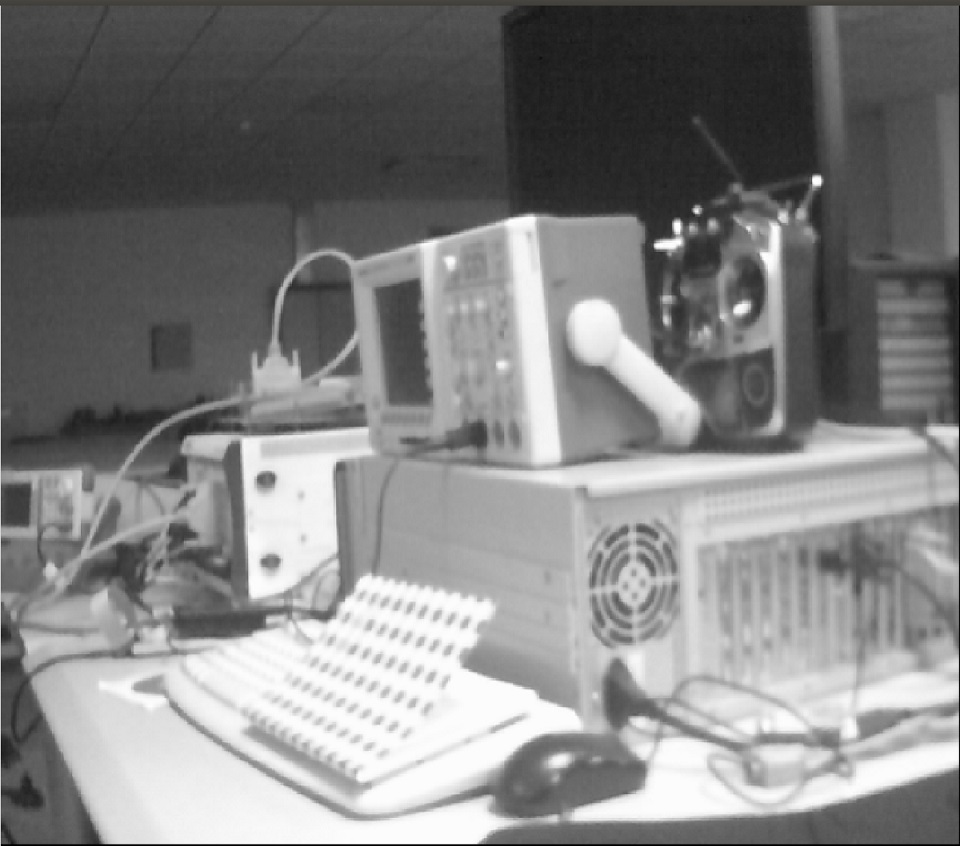
\includegraphics[scale=.2]{figures/Fig4(a)}          
          %\subcaption{}
          }                    
          \subfigure[]
       	  {
          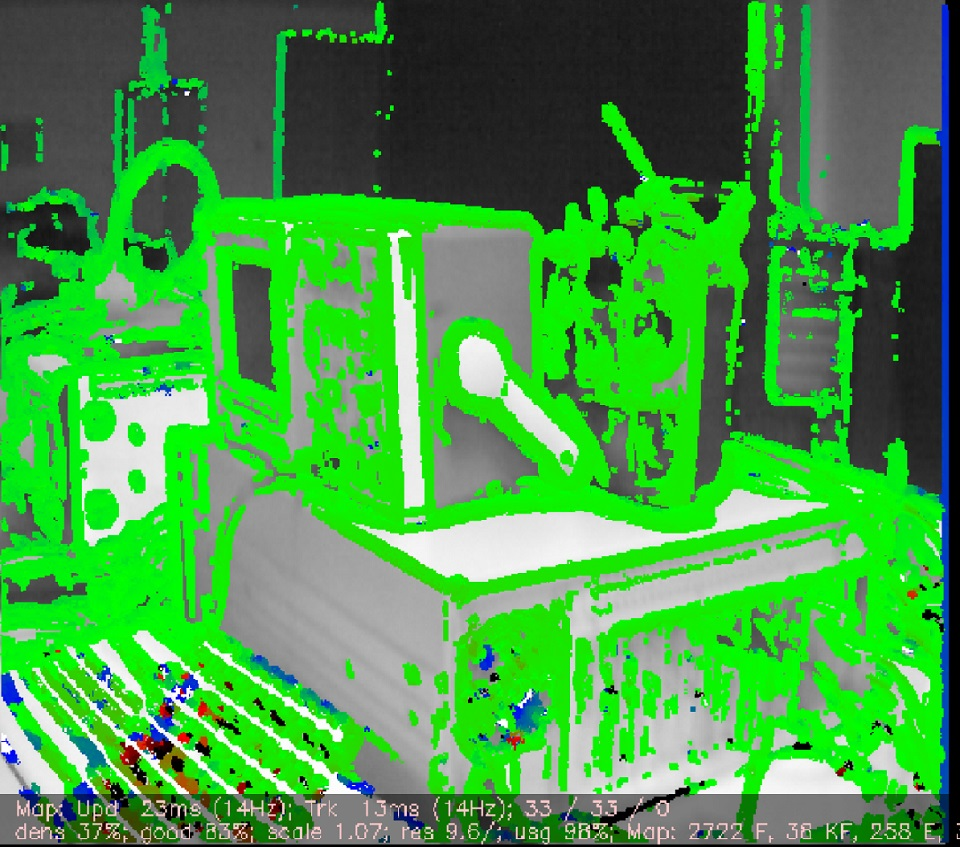
\includegraphics[scale=.2]{figures/Fig4(b)}
          %\subcaption{}
          }
          \hspace{0in}
     
          \subfigure[]
       	  {
          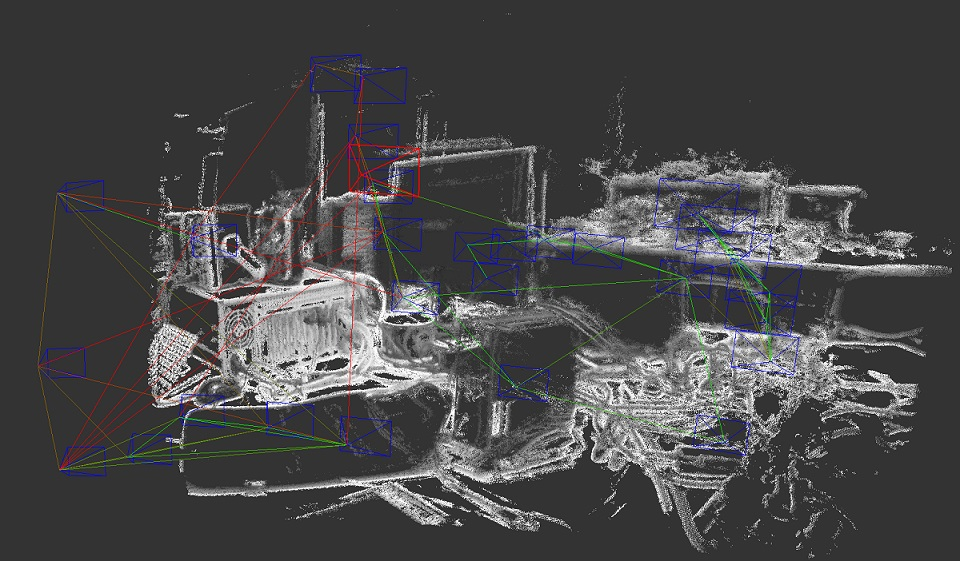
\includegraphics[scale=.25]{figures/Fig4(c)}
          %\subcaption{}
		  }
		  \subfigure[]
       	  {          
          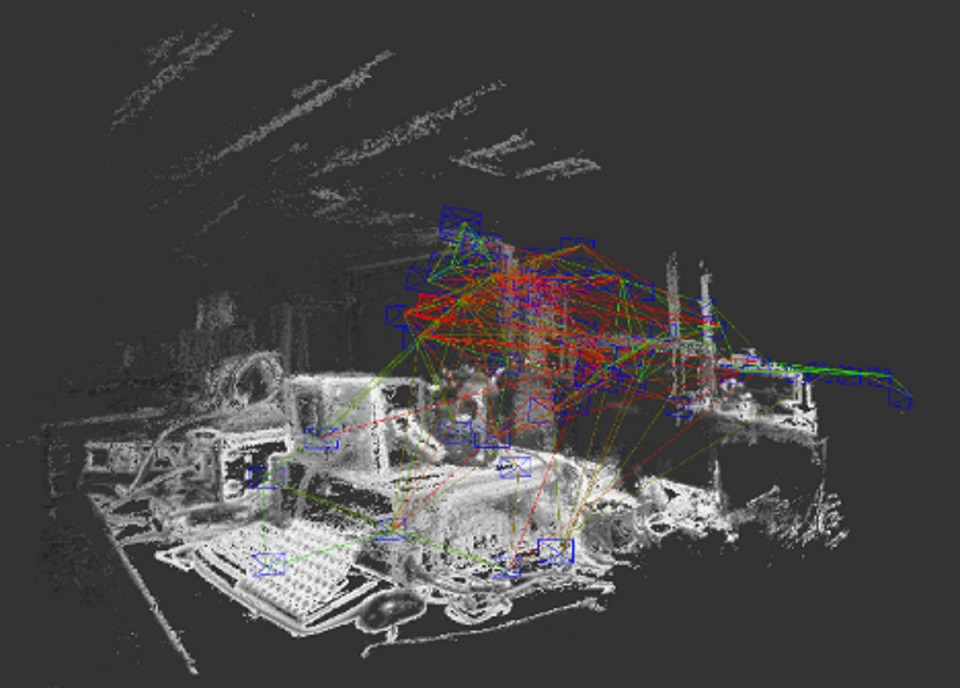
\includegraphics[scale=.2]{figures/Fig4(d)}
          %\subcaption{}
          }
          \hspace{0in}
       %\end{minipage}
     \caption{The indoor LSD-SLAM Map}
\end{figure}

\fi

%4.2
\section{极线搜索与块匹配}
对于当前关键帧$K_i$中像素梯度的模大于$\lambda_G$的像素$p$,会在关键帧$K_j \in K$的极线$l_j$上$\left[ \rho_{min}, \rho_{max} \right]$范围内进行搜索,寻找匹配的像素点,如图\ref{fig4.1}所示。极线利用基本矩阵$F_{ji}$求得,极线搜索方程如下所示。
\begin{equation}
\label{equ4.1}
x_j^T F_{ji}x_p = x^T_jl_j=0 \rightarrow v_j = m \cdot u_j+n
\end{equation}

\begin{figure}
\label{fig4.1}

\end{figure}



\iffalse
We evaluate the LSD-SLAM performance in outdoor. We accomplish the reconstruction the 3D map in diverse scene which is different distance. The result is expressed in Fig.5

The picture (a) and (b) are the different distance scene reference image for hand holding camera. The (c) and (d) is the reconstruction map of the LSD-SLAM. We can find that the mapping is completely reconstructed the scene information and the noisy is low in outdoor environment. This can be used in unmanned aerial vehicle(UAV) navigation and localization. The LSD-SLAM is reliable and robustness.

\begin{figure}
    \centering
       %\begin{minipage}{5cm}
       	  \subfigure[]
       	  {
          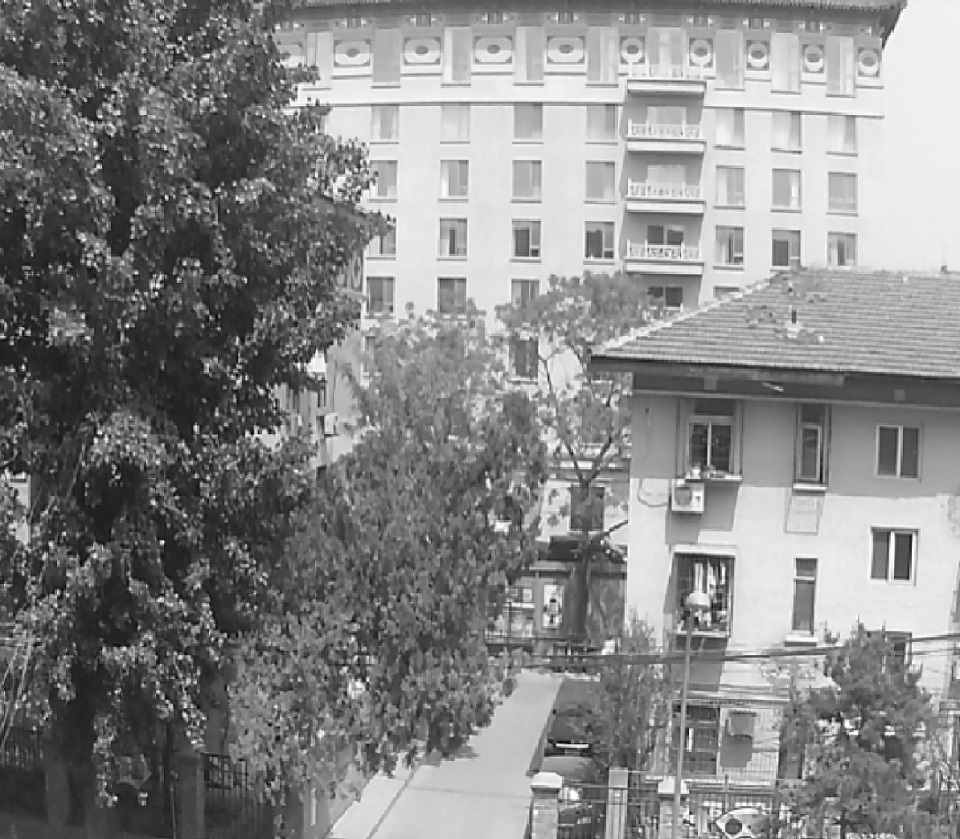
\includegraphics[scale=.2]{figures/Fig5(a)}          
          %\subcaption{}
          }                    
          \subfigure[]
       	  {
          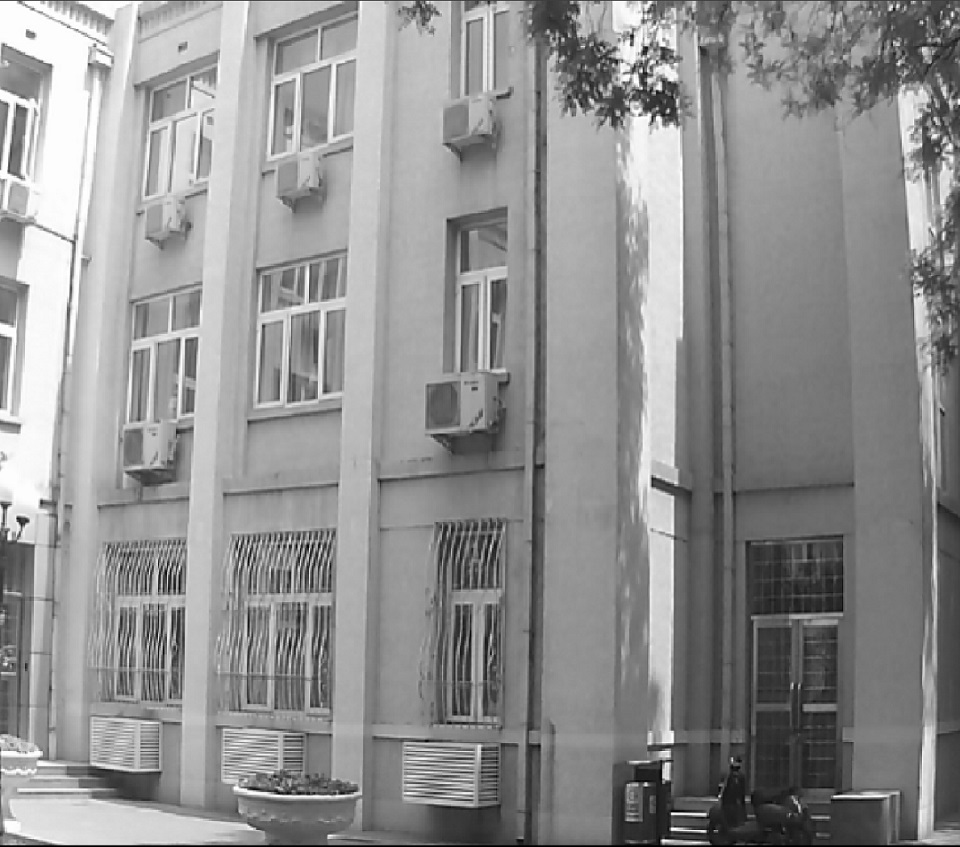
\includegraphics[scale=.2]{figures/Fig5(b)}
          %\subcaption{}
          }
          \hspace{0in}
     
          \subfigure[]
       	  {
          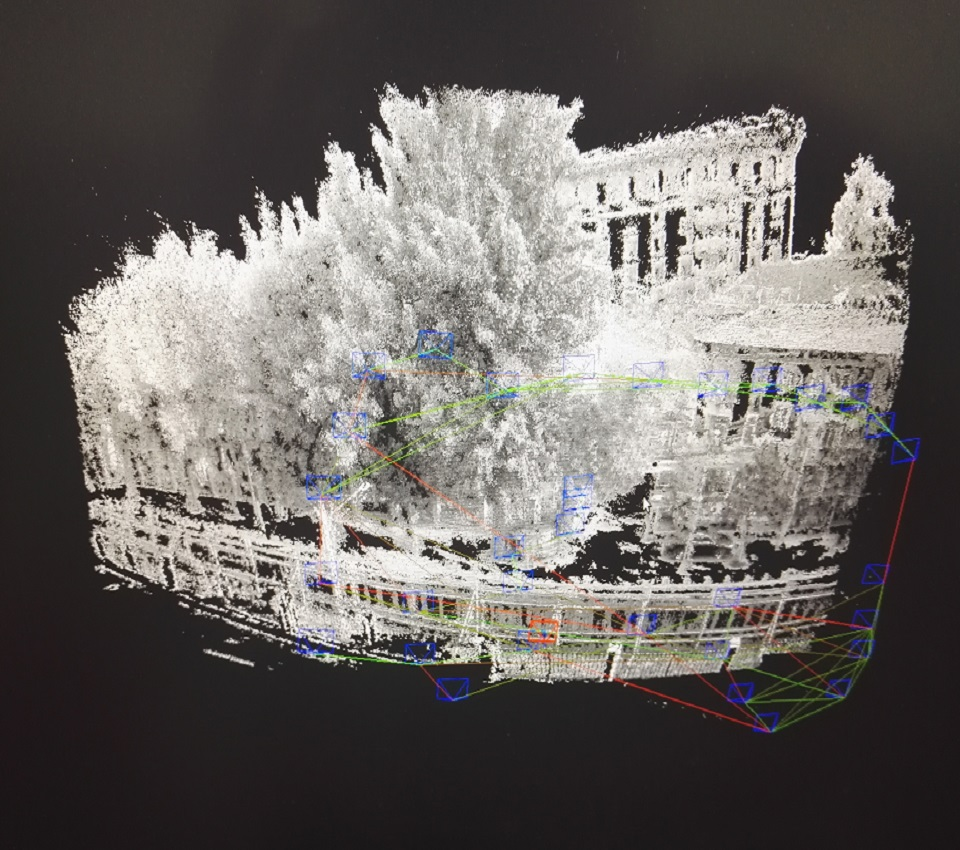
\includegraphics[scale=.25]{figures/Fig5(c)}
          %\subcaption{}
		  }
		  \subfigure[]
       	  {          
          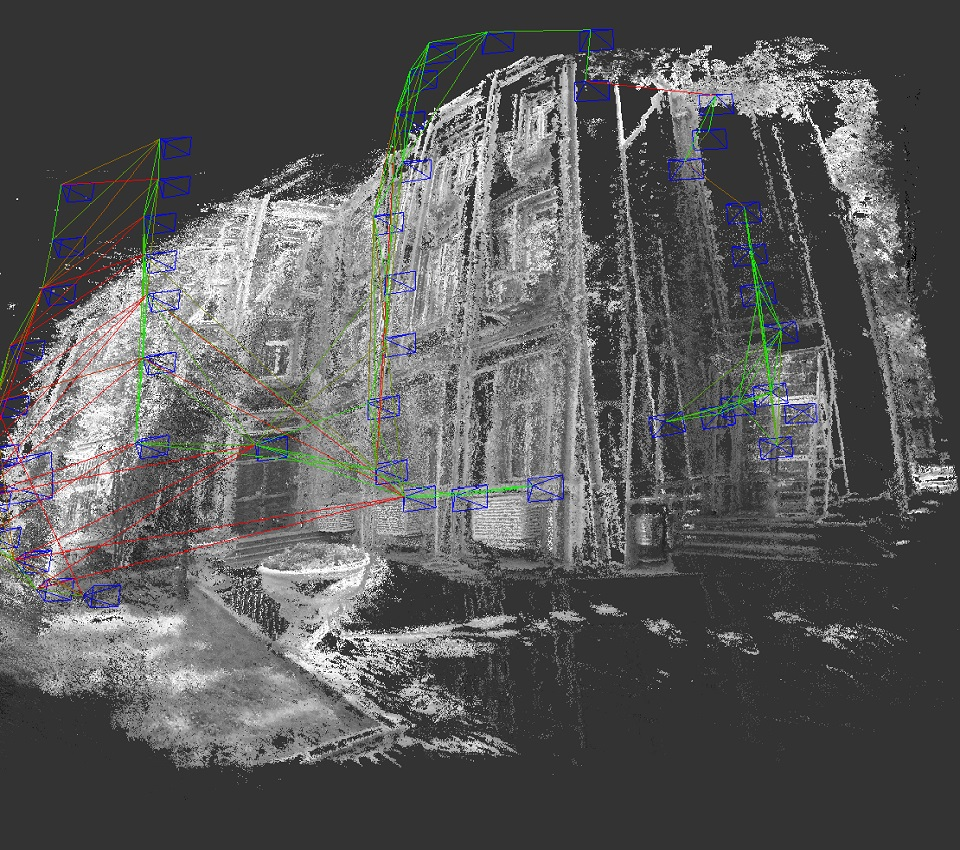
\includegraphics[scale=.2]{figures/Fig5(d)}
          %\subcaption{}
          }
          \hspace{0in}
       %\end{minipage}
     \caption{The outdoor LSD-SLAM Map}
\end{figure}
\fi

%4.3
\section{逆深度假设融合}

\begin{table}
\newcommand{\tabincell}[2]{\begin{tabular}{@{}#1@{}}#2\end{tabular}}
\centering

    \caption{Localization Error in Tum Dataset}     % NOTE!  caption goes _before_ the table contents !!
    \label{tab:font-sizes}
	\renewcommand\arraystretch{1.5}
    \begin{small}
    \begin{tabular}{p{2cm}p{1.5cm}p{1.5cm}p{1.5cm}}
    \hline

    \multicolumn{1}{c}{\multirow{3}{*}{Seq.}}
    & \multicolumn{3} {c} {\bfseries\tabincell{c} {Absolute Key Frame \\ Trajectory RMSE(cm)}} \\
    \cline{2-4}
    \multicolumn{1}{c}{}&   \multicolumn{1}{c}{\bfseries \tabincell{c}{LSD-SLAM} }      &     \multicolumn{1}{c}{\bfseries \tabincell{c}{ semi-dense \\mono-VO}}   & \multicolumn{1}{c}{\bfseries \tabincell{c}{ RGB-D \\SLAM}} \\	

    \cline{1-4}


  \multicolumn{1}{c}{fr2/desk}     &\multicolumn{1}{c}{5.65}      &\multicolumn{1}{c}{13.50}       &\multicolumn{1}{c}{2.58}   \\

  \multicolumn{1}{c}{Fr2/xyz}       &\multicolumn{1}{c}{2.15}      &\multicolumn{1}{c}{3.79}        &\multicolumn{1}{c}{1.34}   \\

  \multicolumn{1}{c}{sim/slowmo}    &\multicolumn{1}{c}{0.37}      &\multicolumn{1}{c}{2.21}        &\multicolumn{1}{c}{0.13}   \\

  \hline

    \end{tabular}
    \end{small}
\end{table}

The LSD-SLAM is evaluated on the Tum dataset. It is very challenging because of containing fast rotational movement, strong motion blur and rolling shutter artifacts. The result is displayed in tableⅠand compared with other algorithm for the localization accuracy.We use the very first depth map to bootstrap the system and get the correct initial scale.

%4.4
\section{帧内逆深度假设一致性检验}



%4.5
\section{帧间逆深度假设一致性检验}


\section{本章小结}

采取了什么方法,针对出现的问题进行优化,表现出了比现有算法更好的性能。

